\documentclass[twocolumn,aps,prl,amsmath,amssymb,longbibliography]{revtex4-2}
\usepackage{graphicx}
\usepackage{dcolumn}
\usepackage{bm}
\usepackage{amsfonts}
\usepackage{xcolor,tabu}
\usepackage{multirow}
\usepackage{amsthm}
\usepackage{textcomp}
\usepackage{tikz}
\usepackage[colorlinks=true,
            linkcolor=blue,
            urlcolor=blue,
            citecolor=blue]{hyperref}
\hypersetup{bookmarksopen=true}
\usepackage{xr}
% Comment type:
  % -- general comments and communications: questions, uncertainties, marks for further considerations, etc.
  %% -- the original sentence
  %%% -- my changes and reason(s) for the change

% modified sentences will be used in the main text.
% comments will be below the modified sentence

% Things to discuss:

\begin{document}

\title{Giant Number Fluctuations and Energy Spectra of 3D Bacterial Suspensions}

\author{Zhengyang Liu}
%\email{liux3141@umn.edu}
\author{Wei Zeng}
\author{Xiaolei Ma}
\author{Xiang Cheng}
\email{xcheng@umn.edu}


\affiliation{Department of Chemical Engineering and Materials Science, University of Minnesota, Minneapolis, MN 55455, USA}

\date{\today}


\begin{abstract}
Giant number fluctuations, a landmark of collectively moving active particles, is universal in active systems across multiple length scales. Here, we present the first experimental study on the giant number fluctuation in 3-dimensional bacterial suspensions. Our measurements show that the number fluctuation scaled by the square root of mean number $\Delta N / \sqrt N$ scales with $N^{0.32}$ at high concentrations, confirming the theoretical predictions. Near the phase boundary, we observe a simultaneous increase of the scaling exponent and the flow induced by bacterial motions, suggesting a strong interplay between giant number fluctuations and flow. We show that this interplay spans all length scales in an active turbulence, by analyzing the kinetic energy spectra.

\end{abstract}

\maketitle

Active fluids exhibit many unusual behaviors beyond the expectation of equilibrium statistical mechanics \cite{Ramaswamy2010,Cates2012,Marchetti2013,Poon2013,Elgeti2015}.
In particular, an active fluid can exhibit anomalously large density variations, the so-called giant number fluctuations (GNF), where the standard deviation of the number of particles grows nonlinearly with the square root of the mean particle number, defying the central limit theorem of equilibrium systems \cite{Mishin2015}.
Such unusual density fluctuations have been observed in a wide range of active fluids in both living and non-living systems including vibrated granular rods \cite{Narayan2007,Aranson2008,Kudrolli2008,Deseigne2010},
swarming bacteria \cite{Zhang2010,Nishiguchi2017} and mammalian cells \cite{Kawaguchi2017},
self-propelled cytoskeleton \cite{Schaller2013}, and synthetic colloidal swimmers \cite{Palacci2013,Karani2019}. As a result, GNF has generally been viewed as a hallmark of the emergent behaviors of active fluids.


Significant theoretical and computational advancement on GNF has been made over the past two decades since the seminal works of Toner and Tu \cite{Toner1995,Tu1998,Toner1998,AditiSimha2002,Ramaswamy2003,Toner2005,Chate2008,Mishra2010,
Dey2012,Saintillan2012,Saintillan2013,Ngo2014,Mahault2019}. Meanwhile, many important theoretical and numerical predictions have been tested in experimental realizations
\cite{Narayan2007, Aranson2008, Deseigne2010, Zhang2010, Schaller2013,
Nishiguchi2017, Kawaguchi2017, Palacci2013}.
%% Although significant progress has been made in the theoretical understanding of GNF over the last two decades since the seminal works of Toner and Tu\cite{Toner1995,Tu1998,Toner1998,AditiSimha2002,Ramaswamy2003,Toner2005,Chate2008,Mishra2010, Dey2012,Saintillan2012,Saintillan2013,Ngo2014,Mahault2019}, quantitative experimental verification of many important theoretical and numerical predictions on GNF is still out of reach.
Of particular interest is the scaling exponent $\alpha$, which is defined following $\Delta N /\sqrt N \propto N^\alpha$, where $\Delta N$ is the standard deviation of particle number and $N$ is the mean number of particles in a subsystem of given size. Heretofore, all the existing experiments on GNF were limited to two-dimensional (2D) or quasi-2D systems. In contrast to theoretical predictions (where $\alpha \approx 0.3$), $\alpha$'s obtained in these experiments show large variations ranging from 0.13 to 0.5. Such a large variation arises partially because of complicated particle-boundary interactions, which are hard to incorporate in theoretical studies. Moreover, the predictions of $\alpha$ in three-dimensional (3D) wet active fluids---one of the most important classes of active fluids where hydrodynamics dominate the interparticle interactions and conserve the total momentum of systems \cite{Marchetti2013}---has not been experimentally testified. Therefore, there is an imperative need for an experimental measurement of $\alpha$ in 3D active fluids, which are not affected by system boundaries. Such a measurement will provide not only an unambiguous experimental benchmark to testify theories of active fluids, but also experimental support on the effect of dimensionality on GNF of active fluids \cite{Marchetti2013}.
%% Here, $\alpha$ is defined following $\Delta N /\sqrt N \propto N^\alpha$, where $\Delta N$ is the standard deviation of particle number and $N$ is the mean number of particles in a subsystem of given size.
%% the mean number of particles of a subsystem of given size
%%% of --> in

%% Heretofore, all the existing experiments on GNF were limited to two-dimensional (2D) or quasi-2D systems\cite{Narayan2007, Aranson2008, Deseigne2010, Zhang2010, Schaller2013, Nishiguchi2017, Kawaguchi2017, Palacci2013}. $\alpha$ obtained in 2D experiments shows large variations ranging between 0.13 and 0.5. Such a large variation arises partially because of complicated particle-boundary interactions, which are hard to incorporate in theoretical studies.
%% In contrast, GNF of bulk 3D active fluids are not affected by system boundaries and therefore provides a better control experimental condition for verifying theoretical predictions.

%%% add an before unambiguous
%% Although theoretical prediction of GNF in 2D systems has also been made \cite{Toner1995,Toner2005}, an experimental consensus of the scaling exponent has not been reached.
%%% Rearranged p2 to save space and avoid repetition


The rise of GNF in active fluids is usually accompanied by the transition to ordered phases with collective motions \cite{Ramaswamy2010,Marchetti2013}. For wet 3D active fluids such as bacterial suspensions, these collective motions lead to large-scale coherent flows with intermittent vortices and jets, which are often referred to as active turbulence \cite{Wolgemuth2008,Wensink2012,Dunkel2013a,Bratanov2015,Guo2018,Linkmann2019,Bardfalvy2019,Alert2020,Skultety2020,Peng2020}. Similar to GNF that manifests density fluctuations across different scales, the flow of active turbulence also exhibits scale-dependent structures. Imported from the study of classical turbulence, energy spectra are frequently measured to quantify such structures in active turbulence \cite{Ishikawa2011,Wensink2012,Dunkel2013a,Giomi2015,Creppy2015,Patteson2018,Alert2020}. Although both GNF and energy spectra quantify the scale-dependent dynamics of active fluids, the deep connection between these two quantities at different scales has not been experimentally investigated. \textcolor{red}{Bridging these two different aspects of active fluids provides new insights into the origin of GNF and reveal hidden dynamic structures of active turbulence.}
% Ths significance statement need further modification

%% frequently measured to quantify such scale-dependent flow properties and to illustrate energy transfer between different scales in active turbulence.
%% Nevertheless, existing experiments on energy spectra of active turbulence all focused on high-concentration suspensions with fully developed active turbulent flows \cite{Ishikawa2011,Wensink2012,Dunkel2013a,Creppy2015,Patteson2018}. How the characteristic turbulent spectrum emerges with increasing particle concentration has not been systematically studied.
%% More importantly, although both GNF and energy spectra quantify the scale-dependent dynamics of active fluids, the intrinsic relation between the two quantities have not been explicitly discussed.

\begin{figure}[ht]
\begin{center}
\includegraphics[width=0.47\textwidth]{Figures/experiment/v5.pdf}
\caption[Experimental details]
{
(a) Active turbulence in a dense bacterial suspension (6.4\%) displaying constantly varying concentration inhomogeneity. Scale bar is 85 \textmu m.
(b) Velocity field of the active turbulence in the dense bacterial suspension ($\phi=6.4\%$) shown in (a).
(c) A dilute bacterial suspension (1.6\%) showing weaker density variations.
(d) Volume fraction as a function of averaged pixel intensities. Inset shows bacterial suspensions of different volume fractions under the same illumination conditions.
}
\label{fig:experiment}
\end{center}
\end{figure}

In this letter, we present our systematic experimental study of GNF and energy spectra in bulk bacterial suspensions, a premier example of 3D wet active fluids. We use genetically engineered light-powered \textit{Escherichia coli} (\textit{E. coli}) as our model bacteria \cite{Liu2020}.
% \textcolor{red}{Some details about the light-control bacteria and the culturing procedure needed to be given in SM.}
For a typical experiment, a bacterial suspension of control volume fraction $\phi$ is injected into a sealed chamber of 20 mm $\times$ 3 mm $\times$ 140 $\mu$m.
Without supply of oxygen, bacteria quickly consume all the remaining oxygen in the chamber and stop moving after $5$ minutes.
We then illuminate the suspension with a high-intensity microscope light, which powers bacteria at their maximal swimming speed of $11 \pm 1$ $\mu$m/s in the dilute limit.
A video of the suspension is taken 50 $\mu$m above the bottom wall of the chamber by a bright-field inverted microscope at a frame rate of $30$ fps and the field of view of $420 \times 360$ $\mu$m$^2$ (Fig.~\ref{fig:experiment}a).
We use a standard Particle Image Velocimetry (PIV) algorithm to extract the 2D in-plane velocity field $(v_x,v_y)$ in the 3D suspension, which exhibits the characteristic chaotically-moving vortices and jets of active turbulence at high $\phi$ (Fig.~\ref{fig:experiment}b).

It is challenging to directly count the number of bacteria in a 3D suspension of fasting moving bacteria. Luckily, the local bacterial density is monotonically correlated with the local intensity of microscope images, where darker regions correspond to higher bacterial densities (Fig.~\ref{fig:experiment}a and Supplementary Video). Such a correlation arises from the Beer-Lambert law, the working principle of spectrophotometry \cite{Tortora2018}, which has already been exploited in probing the dynamics in suspensions of bacteria and actin filaments \cite{Sokolov2009, Wilson2011, Schaller2013}.
%Such a correlation derived from the Beer-Lambert law forms the basis of spectrophotometry routinely used in microbiology in measuring bacterial density \cite{Tortora2018} and has also been exploited previously in probing the dynamics in suspensions of bacteria and actin filaments \cite{Sokolov2009, Wilson2011, Schaller2013}.
%Note that the length scale of dense dark clusters is much smaller than the height of the chamber.
% On the macroscopic scale of the chamber, the light intensity is still uniform. \textcolor{red}{This is argument is wrong if the microscopy light is the same as the light power light.} Moreover, the life time of the dense clusters is significantly shorter than the response time of bacteria to the change of light condition. Hence, the motility of light-powered bacteria should not be affected by the local fast light attenuation and is dominantly controlled by the average intensity of illuminating light. \textcolor{red}{We need to justify the formation of clusters does not strongly affect bacteria motility, since in the clusters the light is dimmer. The other argument could be we already saturate the light response of bacteria. Even though in the clusters light is dimmer, bacterial motility is still the same.}
To calibrate the density-intensity correlation, we prepare bacterial suspensions of different $\phi$ and image the suspensions under the same illumination (Fig.~\ref{fig:experiment}c inset). The mean image intensity decreases with increasing $\phi$ following an approximately linear relation (Fig.~\ref{fig:experiment}c), agreeing with the the Beer-Lambert law for samples of small thickness and weak absorptivity appropriate for our experiments. The linear density-intensity relation has also been used in previous experiments on \textit{E. coli} suspensions \cite{Wilson2011}.


\begin{figure}[ht]
\begin{center}
\includegraphics[width=0.47\textwidth]{figures/spatiotemporal-correlations/v3.pdf}
\caption[spatiotemporal-correlations.]
{
(a-c) Velocity and concentration spatial correlation functions $C_{v}(r)$  and $C_{n}(r)$ and correlation lengths $\lambda$,
(d-f) Velocity and concentration temporal autocorrelation functions $C_{t, v}(t)$  and $C_{t, n}(t)$ and correlation times $\tau$ at volume fractions ranging from 0.8\% to 9.6\%.
}
\label{fig:spatiotemporal-correlations}
\end{center}
\end{figure}

\begin{figure}[ht]
\begin{center}
\includegraphics[width=0.47\textwidth]{figures/GNF/v3.pdf}
\caption[Concentration dependence of GNF.]
{
\textbf{Concentration dependence of GNF.}
Standard deviation of particle number $\Delta N$ scaled by particle mean number $N$ plotted against subsystem size rescaled by single bacterium size $l^2/l_b^2$ in bacterial suspensions at volume fractions ranging from 0.8\% to 9.6\%. Shaded region indicates the range over which the scaling exponents $\alpha$ are fitted.
Inset: Concentration dependence of the scaling exponents $\alpha$. Dashed line indicates the high concentration plateau value of $\alpha$ which equals approximately $0.30 \pm 0.01$.
}
\label{fig:GNF}
\end{center}
\end{figure}


\textit{Density fluctuations.}--The simple linear relation allows us to measure the spatiotemporal evolution of relative local bacterial densities and investigate density fluctuations in 3D bacterial suspensions. We first calculate the two-point density spatial correlation and the density auto-correlation for suspensions of different $\phi$ and compare them with well-studied velocity correlations extracted from PIV \cite{Liu2020}.
%% \textcolor{red}{Should we also show autocorrelation? We could have a separate figure for all the four correlations (density, velocity, spatial and auto). In any case, we need to show the definition of the correlation function(s) in SM, if not here in the main text.}
%%%%%%% Done in SM
The correlation length $\lambda$ and correlation time $\tau$ are determined when the corresponding normalized correlation functions decay to $1/e$. Fig.~\ref{fig:experiment}d shows the density correlation lengths at different $\phi$, which characterize the scale of density inhomogeneities in suspensions.
%% \textcolor{red}{(use a symbol different from $l$ for the correlation length, e.g. $\lambda$, since $l$ is used as the size of subsystem below)}
%%%%%%%%%%%%%%% use \lambda: done
$\lambda$ is small at low $\phi$, gradually increases with $\phi$ and reaches a plateau of $\sim 5l_b$ in high-concentration bacterial suspensions of $\phi > \phi_c = 3.5\%$, where $l_b=3$ $\mu$m is the average length of bacterial body. The velocity correlation length follows the exact same trend and also saturates when $\phi > \phi_c$. Such a quantitative similarity indicates the direct coupling between density fluctuations and collective turbulent flows, a feature we shall examine in much more details later. In the fully-developed turbulent regime above $\phi_c$, the velocity correlation length is about twice of the density correlation length.
%% \textcolor{red}{If we show auto-correlation, we need to discuss the correlation time too. The correlation time could be important to justify the 10 frames used in your analysis below.}
%%%%%%% Discuss: autocorrelation is included in SI,

We further examine GNF by calculating the standard deviation of bacterial number $\Delta N$ and the mean bacterial number $N$ in subsystems of increasing sizes \cite{Liu2020}. $\Delta N / \sqrt N$ as a function of $l^2/l_b^2$ for bacterial suspensions of different $\phi$ is plotted in Fig.~\ref{fig:GNF}a, where $l$ is the side length of square subsystems. Note that the area of the subsystem $l^2$ is linearly proportional to mean particle number $N$ at given $\phi$. At low $\phi<\phi_c$ where bacterial suspensions do not show clear active turbulence, $\Delta N$ scales linearly with $\sqrt N$, resulting in constant $\Delta N / \sqrt N$ independent of subsystem sizes. Above $\phi_c$, bacterial suspensions transition into active turbulence \cite{Peng2020}, where $\Delta N$ increases faster than $\sqrt N$, showing the defining feature of GNF.

The degree of GNF can be quantified by the scaling exponent $\alpha$ following $\Delta N/\sqrt{N} \sim N^\alpha$. $\alpha=0$ for equilibrium systems obeying the central limit theory, whereas the upper bound $\alpha = 0.5$ corresponds to a system with maximal density fluctuations. When the size of subsystems is much larger than the density correlation length $\lambda$, the giant fluctuation diminishes due to the spatial average over multiple dense and dilute regions (Fig.~\ref{fig:GNF}a). Hence, to extract $\alpha$, we fit the experimental curves with power-law relations only in the short length limit between $3.5l_b$ to $12 l_b$. Fig.~\ref{fig:GNF}b shows $\alpha$ as a function of $\phi$. $\alpha$ remains small at low $\phi$ when the swimming of bacteria is random and increases sharply above $\phi_c$ when bacterial suspensions show active turbulence with saturated correlation lengths (Fig.~\ref{fig:experiment}d).
$\alpha$ approaches to a high plateau of $0.32 \pm XX$ at even higher $\phi \geq \phi_h = 6.4\%$. The plateau value quantitatively agrees with the theoretical prediction of $\alpha = 1/3$ for 3D suspensions of polar-ordered self-propelled particles with hydrodynamic interactions \cite{AditiSimha2002}. \textcolor{red}{Please provide the error bar.} As such, our experiments provide the first quantitative verification of the theory of GNF in 3D wet active fluids. Nevertheless, the gradual increase of $\alpha$ at intermediate $\phi$ between $\phi_c$ and $\phi_h$ where active turbulence has already been established cannot been explained by the linear theory. Such a gradual increase has been observed in numerical simulations of suspensions of self-propelled rods beyond the linear regime \cite{Saintillan2012}.

\begin{figure}[!]
\begin{center}\includegraphics[width=0.47\textwidth]{Figures/energy-spectra/v3.pdf}
\caption[Concentration dependence of energy spectra.]
{
Energy spectra of bacterial active turbulence at volume fractions ranging from 0.8\% to 9.6\%. Shaded region indicates the range over which the scaling exponents $\beta$ are fitted. Red dashed line is a fitting of the $\phi=0.8\%$ curve (purple), based on the hydrodynamic model of Ref.~\cite{Bardfalvy2019}. Fitting parameters: $n=0.07\%$ and $\epsilon=98$.
Inset: Scaling exponents of energy spectra ($\beta$) as a function of volume fractions $\phi$. Dashed line is $3.3 \pm 0.1$.
}
\label{fig:energy-spectra}
\end{center}
\end{figure}

\textit{Energy spectra.}--
Similar to GNF, the velocity field of active turbulence also shows scale-dependent structures, which are often characterized by the energy spectrum of turbulent flows, $E(k)$ \cite{Liu2020}. $E(k)$ measures the kinetic energy density at different scales in terms of wavenumber $k = 2\pi/l$. It is related to the mean kinetic energy density $E = \langle v_x^2 + v_y^2 \rangle/2$ via $E = \int_0^\infty E(k)dk$. Fig.~\ref{fig:energy-spectra}a shows $E(k)$ of bacterial suspensions at different $\phi$.
%% \textcolor{red}{We should plot $k/k_b$, instead of $k$ in analogy of $l/l_b$ for GNF.}
%%%%%%%%%%%%% Done
At low $\phi$ with random swimming bacteria, $E(k)$ quantitatively agrees with the theoretical prediction for uncorrelated pusher swimmers \cite{Bardfalvy2019}
\begin{equation}
E_k = 4\pi n \kappa^2 \left[ \frac{1}{3} + \frac{\cos(kl)}{(kl)^2} - \frac{\sin(kl)}{(kl)^3} \right] \frac{\epsilon^4k^2}{l^2} K_2^2(k\epsilon)
\end{equation}
where  $\kappa \approx 400$ $\mu$m$^3$/s is the dipole strength of \textit{E. coli}, $l\approx 1.9$ is the dipolar length, $\epsilon$ is a factor describing the distance over which the regularisation acts and $K_2$ is the modified Bessel function of the second kind. The fitting parameters $n$ and $\epsilon$ are found to be 0.07\% and 98, respectively.
%%\textcolor{red}{Show the fitting equation and explain the meaning of the symbols.}
%%%%%%%%%%%%%% Confused about units, check the paper
Particularly, $E(k)$ is flat in the small $k$ limit, a feature arising from the superposition of the dipolar flow fields of uncorrelated bacteria \cite{Bardfalvy2019}.
%%%%%%%%%%%%% Discuss: I don't understand
%% \textcolor{red}{The theory shows $E(k) = 8\pi/15 n \kappa^2$ in the low $k$ limit, where $\kappa = Fl/\eta$ with $Fl$ the dipole strength and $\eta$ viscosity. Does this prediction quantitatively agree with our measurements?}
%%%%%%%%%%%%% Discuss: I don't think it's a low k prediction.
%% $E(k)$ at small $k$ increases with $\phi$.
With increasing $\phi$, $E(k)$ at small $k$ increases sharply. In the turbulent regime at high $\phi$, the kinetic energy is all concentrated at scales much larger than the size of single bacteria $l_b$, even though the turbulent flows are completely powered by single bacterial swimming at $l_b$.
Weak peaks are observed for high $\phi$ suspensions at low $k$. This overall trend of $E(k)$ with increasing $\phi$ qualitatively agrees with large-scale simulations \cite{Saintillan2012,Bardfalvy2019}.

We also extract the scaling exponent $\beta$ from $E(k) \sim k^{-\beta}$ by fitting the energy spectra at intermediate and large $k$, where a significant change of $E(k)$ with $\phi$ occurs and $E(k)$ exhibits good power-law relations.
%% \textcolor{red}{I think we should use a smaller range of $k$ in the fitting. For the low $\phi$ samples, the curves are apparently nonlinear in the current range.I don't think we need to enforce the overlap of the length scales between GNF and energy spectra at this point, since we will plot $\Delta N/\sqrt{N}$ and $E(k)$ directly anyway.}
%%%%%%%%%%%%%%% Sure
Similar to the trend of $\alpha$, $\beta$ also increases with $\phi$ and saturates at $2.9 \pm 0.1$ at high $\phi \geq \phi_h$. The saturated scaling exponent is quantitatively the same as that of the active turbulence of high-concentration suspensions of sperm at large $k$ \cite{Creppy2015}.
The exponent is also consistent with experiments on confined dense suspensions of \textit{B. subtilis} and swarming \textit{S. marcescens} on agar substrates, where the scaling of $E(k) \sim k^{-8/3}$ has been reported at large $k$ \cite{Wensink2012,Patteson2018}. Since the characteristic vortex size quantified by the velocity correlation length is linearly proportional to the system size $L$ \cite{Guo2018}, when $k$ is significantly smaller than $2\pi/L$, $E(k)$ would decreases, exhibiting the non-monotonic trend shown in \cite{Wensink2012,Patteson2018}. The large system size of $L = 140$ $\mu$m of our experiments allows us to probe the small $k$ limit predicted by theories and simulations without the influence of system boundaries.

Although the scaling in the small $k$ limit is strongly affected by the system size, the scaling in the large $k$ limit seems to be universal with $\beta \approx 3$ from different experiments. To the best of our knowledge, no theoretical prediction has been made on this interesting scaling behavior for 3D wet active fluids. Giomi investigated the energy spectra of 2D active nematics by combining numerical simulations with mean-field theories and showed $E(k) \sim k^{-4}$ in the large $k$ limit \cite{Giomi2015}.
The result has also been confirmed recently by a hydrodynamic theory \cite{Alert2020}. For isotropic turbulence in $d$ dimension, the energy spectra can be written as $E(k) = C_d k^{d-1} \langle \mathbf{v}(\mathbf{k})\cdot \mathbf{v}(-\mathbf{k})\rangle_{k = |\mathbf{k}|}$ \cite{Wensink2012,Bardfalvy2019},
where $C_d k^{d-1}$ is the surface area of $d$-sphere and $\langle \mathbf{v}(\mathbf{k})\cdot \mathbf{v}(-\mathbf{k})\rangle_{k = |\mathbf{k}|}$ is the Fourier transform of the velocity-velocity spatial correlation function. If we assume that the velocity correlation function for 2D active nematics is quantitatively similar to that of 3D bacterial suspensions independent of the dimensionality of systems, the mean-field theory would then predict the correct scaling of $E(k) \sim k^{-3}$ for 3D active turbulence. This hypothesis is certainly highly non-trivial and needs further theoretical investigation. Note that although we measure the energy spectra of 2D in-plane flows of 3D suspensions, the scaling of the spectra is the same as the spectra of 3D turbulent flows \cite{Pope2000}. Taken together, our study provides the first systematic experiments on the evolution of $E(k)$ over a large range of $\phi$ in bulk bacterial suspensions. The results quantitatively verify the existing theory on low-concentration active fluids and serve as a crucial benchmark for future theoretical development on the spectral properties of 3D active turbulence.

\begin{figure}[!]
\begin{center}
\includegraphics[width=0.47\textwidth]{figures/GNF-energy-spectra-correlation/v4.pdf}
\caption[The correlation between GNF and kinetic energy and kinetic energy spectra.]
{
\textbf{The correlation between GNF and kinetic energy and kinetic energy spectra.}
(a) Energy spectra $E$ plotted against number fluctuations ($\Delta N/\sqrt N$) at corresponding length scales at volume fractions ranging from 0\% to 9.6\%. Black arrow indicates the direction of increasing length scale. Inset: the scaling exponent of number fluctuations $\alpha$ plotted against the scaling exponent of energy spectra $\beta$ at corresponding volume fractions. Dashed line has slope $0.08 \pm 0.01$.
(b) Local correlations between density fluctuations and kinetic energy at volume fractions ranging from 0\% to 9.6\%. Inset: a snapshot of a density fluctuation field and a kinetic energy field. The correlations are calculated by averaging over 1000 frames.
}
\label{fig:GNF-energy-spectra-correlation}
\end{center}
\end{figure}

\textit{Density-flow coupling.}--Both GNF and energy spectra probe the scale dependence of active turbulence. The former measures density fluctuations at different scales, whereas the latter considers flow energies across scales. Although both properties have been extensively studied, the coupling between the two has not been explicitly examined so far. The scaling exponents of GNF and $E(k)$ show qualitatively similar increasing trend and both saturate at high $\phi \geq \phi_h$. We plot $\alpha$ versus $\beta$ at different $\phi$ (Fig.~\ref{fig:GNF-energy-spectra-correlation}b inset), which shows a $\phi$-independent constant ratio $\alpha/\beta = 0.087 \pm 0.012$ in the turbulent regime. The finding suggests that a density-independent correlation between density fluctuations and kinetic energies may exist across all different length scales.
Indeed, when we plot density fluctuations $\Delta N/\sqrt N$ against the corresponding kinetic energies $E$ at the same scale, all the $\Delta N/\sqrt N$-$E$ pairs fall onto a universal curve over two orders of magnitude in scales extending from the size of single PIV boxes to the entire field of view of experiments in the active turbulence regime, regardless of the specific volume fractions of the samples. In contrast, $\Delta N/\sqrt N$-$E$ shows much larger scattering for low $\phi$ suspensions with random swimming bacteria. Although it is not surprising that density fluctuations correlate with kinetic energies in general as both measure different aspects of the same active turbulence, the collapse of data and the constant ratio of $\alpha/\beta$ are still quite unexpected. The results show that the coupling between density fluctuations and turbulent flows occur at every scale of active turbulence in a quantitative same fashion. Such a scale-invariant coupling is independent of the volume fraction of bacterial suspensions and manifests even in the turbulent regime between $\phi_c$ and $\phi_h$ where the linear theory fails. Since Newtonian fluids are generally considered to be incompressible, this scale-invariant density-flow coupling does not have an analogue in classical turbulence and is unique to active turbulence.

To further illustrate such an unusual coupling in real space, we measure the \emph{local} correlation of density fluctuations and kinetic energies at a randomly chosen small scale of $l = 5\l_b$. The local density fluctuation $\delta N(\mathbf{r},t)$ and local kinetic energy $E(\mathbf{r},t)$ at position $\mathbf{r} = (x,y)$ and time $t$ are extracted from the image intensity field and the PIV velocity field, respectively (Fig.~\ref{fig:GNF-energy-spectra-correlation}a inset) \cite{Liu2020}. The normalized correlation between $\delta N(\mathbf{r},t)$ and $E(\mathbf{r},t)$ is then computed at different $\phi$ (Fig.~\ref{fig:GNF-energy-spectra-correlation}a). At low $\phi$ with random swimming bacteria, the correlation is weak fluctuating around zero, which then increases with $\phi$ as bacterial suspensions transition to active turbulence. A constant positive correlation is found in the turbulent regime when $\phi \geq \phi_c$. The real-space measurement provides a concrete example of the coupling between density fluctuations and turbulent flows at small scales.

\begin{figure}[!]
\begin{center}
\includegraphics[width=0.47\textwidth]{figures/GNF-energy-spectra-correlation-transient/v1.pdf}
\caption[The correlation between GNF and kinetic energy and kinetic energy spectra at transient state]
{
(a) Evolutions of GNF scaling exponent $\alpha$ (black), flow kinetic energy $E$ (orange) and coherent flow fraction $M$ (blue) during the onset of active turbulence ($\phi=6.4$).
(b) Kinetic energy and number fluctuations at corresponding time and length scales during the onset of active turbulence at volume fractions ranging from 2.4\% to 9.6\%.
}
\label{fig:GNF-energy-spectra-correlation-transient}
\end{center}
\end{figure}

Even more surprisingly, % avoid "surprisingly"
we find that the same density-independent coupling also manifests in the kinetic process during the transition towards bacterial turbulence. Taking the advantage of the light-powered bacteria, we trigger the onset of bacterial turbulence by suddenly turning on the light illumination on high-concentration bacterial suspensions at $t=0$ \cite{Peng2020}. The density fluctuations and the energy spectra are then monitored as a function of $t$ before the suspensions reach the steady turbulent state. First, at the large scale of the system, the emergence of GNF is directly coupled with the increase of the total kinetic energy of the flows (Fig. XXa). Both are significantly delayed compared with the formation of collective flows. Here, we quantify the formation of collective flows by the area fraction of the regions with strong alignment of local velocities \cite{Liu2020,Peng2020}. The finding provides strong experimental support to an important prediction of the kinetic theory of active fluids \cite{Saintillan2008a,Saintillan2008b}, where the density fluctuation arises due to the nonlinear coupling between collective flows and particle densities. At the onset of hydrodynamic instability in the linear regime, the density should stay uniform as confirmed by our experiments at early times.
More importantly, we also analyze the temporal evolution of $\Delta N/\sqrt N$ and $E(k)$ for bacterial suspensions of different $\phi$. All the data at different $t$ and $\phi$ collapse into the same master curve obtained from the steady-state measurements (Fig. XXb) \cite{Liu2020}.
This remarkable result from the kinetic measurements further suggests that the rise of GNF is governed by the kinetic energy at each corresponding scale.
%% Specifically, we divide the images of bacterial suspensions into small square windows of $5.7l_b$. The standard deviation of the density of each window at time $t$, $\delta N(\mathbf{r},t)$, is then calculated over a small time interval of 0.3 s, less than the correlation time of density fluctuations $\tau$. $\delta N(\mathbf{r},t)$ quantifies the local density fluctuation at position $\mathbf{r} = (x,y)$ and time $t$ (Fig.\ref{fig:GNF-energy-spectra-correlation}a inset). The same windows are then also used in PIV to extract the local velocities of bacterial suspensions. The local kinetic energy at $t$ is given by $E_l(\mathbf{r},t) = \left[ V_x(\mathbf{r},t)^2 + V_y(\mathbf{r},t)^2 \right]/2$ (Fig.\ref{fig:GNF-energy-spectra-correlation}a inset). Finally, we calculate the normalized correlation between $\delta N(\mathbf{r},t)$ and $E_l(\mathbf{r},t)$, $C$ for bacterial suspensions of different $\phi$ (Fig.\ref{fig:GNF-energy-spectra-correlation}a).

In summary, we present the first measurement on GNF in 3-dimensional bacterial suspensions. The scaling exponents $\alpha$ we measure are not subject to the effect of frictional walls and are thus more suitable for quantitatively testing theoretical predictions.
Our detailed analysis on the velocity fields reveals a strong coupling between flow kinetic energy and GNF, not only on the global scale, but spans all the length scales down to single swimmer length.
Our measurements will contribute to the advancement of quantitative understanding of collective motions and GNF in bacterial active turbulence.

\bibliographystyle{apsrev4-2}
\bibliography{correlation}

\end{document}
